\section{实验}
\label{sec:experiment}

\begin{table*}[t]
\footnotesize
\caption{ Quantitative comparison of different VSR methods. The results marked with ∗ achieve similar performance as no alignment. This is due to the vanishing of optical flow in this experiment.}
\centering
\resizebox{\textwidth}{!}{
    \begin{tabular}{c|l|ll|cc|cc}
        \toprule
        Exp. &
        \multirow{2}{*}{Method} &
        \multirow{2}{*}{Alignment} & \multirow{2}{*}{Remark} & \multicolumn{2}{c|}{Vimeo90K-T} & \multicolumn{2}{c}{REDS4}\\
        Index & & & & PSNR & SSIM & PSNR & SSIM\\
        \midrule
        1 & VSR-CNN & Image alignment & Finetune flow & 36.13 & 0.9342 & 29.81 & 0.8541\\
        2 & VSR-CNN & No alignment &  & 36.24 & 0.9359 & 28.95 &  0.8280\\
        3 & VSR Transformer & Image alignment & Fix flow  & 36.87 & 0.9429 & 30.25 & 0.8637\\
        4 & VSR Transformer & Image alignment & Finetune flow & 37.44$^*$ & 0.9472$^*$ & 30.43 &  0.8677\\
        5 & VSR Transformer & Feature alignment & Finetune flow & 37.36 & 0.9468 & 30.74 & 0.8740\\
        6 & VSR Transformer & No alignment & Window size 8 & 37.43 & 0.9470 & 30.56 & 0.8696\\
        7 & VSR Transformer & No alignment & Window size 16 & 37.46 & 0.9474 & 30.81 & 0.8745\\
        \bottomrule
    \end{tabular}}
    \label{tab:tab1}
\end{table*}

可以看到,在Image上面使用Patch Alignment就已经可以达到现在最好的一个效果,而且节省了将近2~3兆的参数量。在Feature的层面进行Patch Alignment,达到31.17。

在主流Benchmark上的结果证明了该方法是有效的,在Recurrent只使用六帧进行训练时,能拿到31.88的成绩,使用16帧进行训练时,在REDS上能拿到32.72的成绩。

一些可视化的结果也证明了,例如车牌低分辨率的版本几乎什么都不剩了,但是结合近邻帧可以对它进行一个非常好的重建。可以看到本文的方法是可以把大楼的条纹和窗户给重建出来的。

\begin{figure*}[!htbp]
	\centering
	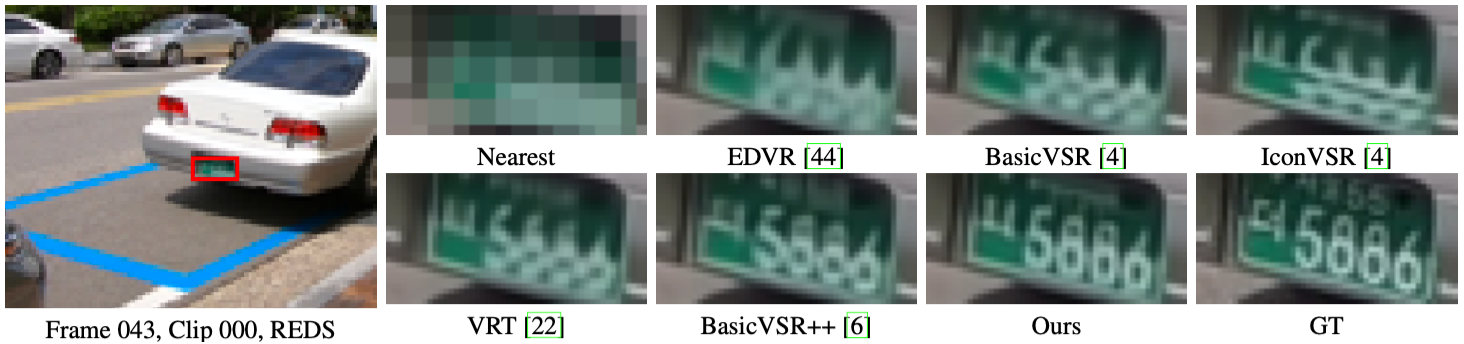
\includegraphics[width=\linewidth]{17.png}
	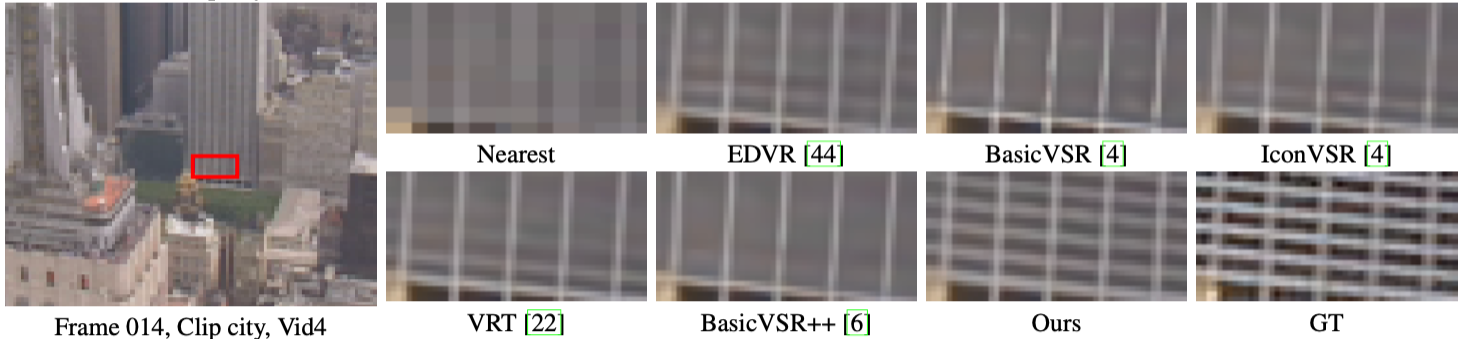
\includegraphics[width=\linewidth]{18.png}
	\caption{VSR (×4) 可视化结果}
\end{figure*}
